\documentclass[conference]{IEEEtran}
\IEEEoverridecommandlockouts


\usepackage{cite}
\usepackage{amsmath,amssymb,amsfonts}
\usepackage{graphicx}
\usepackage{textcomp}
\usepackage{xcolor}
\usepackage{booktabs}
\usepackage{multirow}
\usepackage{array}
\usepackage{url}
\usepackage{tikz}
\usepackage{pgfplots}
\pgfplotsset{compat=1.16}
\usetikzlibrary{shapes.geometric,arrows.meta}


\graphicspath{{figures/}}


% Uses the PNG if it exists in figures/, otherwise draws a labelled placeholder box
\newcommand{\figorbox}[3]{%
  \IfFileExists{figures/#1}%
    {\includegraphics[width=#2]{#1}}%
    {\fbox{\parbox[c][3.4cm][c]{\dimexpr#2-2\fboxsep-2\fboxrule\relax}{\centering\footnotesize TODO: #3\\(\texttt{figures/\detokenize{#1}})}}}}


\def\BibTeX{{\rm B\kern-.05em{\sc i\kern-.025em b}\kern-.08em
    T\kern-.1667em\lower.7ex\hbox{E}\kern-.125emX}}


\begin{document}


\title{When Is Reuse Safe? Regime-Aware Policy Transfer for Recurring Drift in Network Telemetry}


\author{\IEEEauthorblockN{Anonymous Submission}\\
\IEEEauthorblockA{Paper under double-blind review}}


\maketitle


\begin{abstract}
Network telemetry drifts, and the standard fix, retraining, pays the full cost of
rebuilding the model every time. But network regimes recur: a congestion profile, a radio
configuration or an operator comes back. We ask whether a policy learned for a regime can
be reused when that regime returns, and when doing so is safe. Regime-Aware Policy
Transfer (RAPT) stores one ensemble policy per regime, retrieves it on recurrence, and
refits it when rolling accuracy shows it no longer fits. On four network streams under a
strict prequential protocol and thirty seeds, RAPT uses 64--91\% less adaptation CPU than
full retraining. Its macro-F1 is lower than full retraining on all four streams,
significantly so on all four. The clearest failure is UGR'16, where regime identifiers
recur but the feature-to-label mapping does not. Identity-only reuse drops macro-F1 below
even the frozen baseline ($0.914$ against $0.969$). We add RAPT-Guard, which scores the
stored policy and the prefix policy on the most recent labelled window before every reuse
and takes the stored policy only when it wins by a margin. On three of the four streams Guard matches or beats the frozen baseline; on UGR'16 it
recovers most of the loss ($0.936$ against $0.969$) while remaining below it. Across all
four streams its adaptation CPU is 43--81\% below full retraining. Reuse keyed on regime
identity alone is therefore unsafe, and a cheap validation gate removes most of the
damage but not all of it.
\end{abstract}


\begin{IEEEkeywords}
concept drift, network telemetry, online learning, adaptive ensembles, regime-aware
learning, computationally efficient adaptation
\end{IEEEkeywords}


\section{Introduction}
Network monitoring data does not stay the same for long. Load, radio conditions,
subscriber mobility and configuration changes move the distribution, so a classifier
fitted on a period of a 5G testbed or an ISP netflow archive will not stay accurate.
Retraining once performance drops is the standard answer. It works, but it is paid for
again every time, and with high-rate telemetry the total spent rebuilding models can
exceed what it costs to serve predictions. Lightweight detection frameworks for
constrained devices already exist \cite{9427288}, and many detectors decide \emph{when}
to adapt
\cite{bifet2007learning,page1954continuous,gama2004learning,baena2006early,ross2012exponentially,dos2016fast,brockhoff2020time},
but they make no use of how the change is structured. Conditions in networks often come
back: a weekday congestion profile, a radio configuration or an operator-specific QoS
regime may go away and return later. Some of the earliest work in the field was driven by
recurring concepts \cite{schlimmer1986incremental,widmer1994combining}, yet the usual
practice is still to learn again from scratch, even though the model being thrown away
may well be the right one.

The question we ask is whether the discarded information can be kept and used. RAPT keeps
a repository of adaptation policies, each indexed by an operating regime. At a regime
boundary it looks up whether the incoming regime already has a stored policy. When it
does, that ensemble is retrieved at close to zero adaptation cost; when it does not, a
new policy is trained and added to the repository. Since a retrieved policy can be wrong
if the label relationship in that regime has changed, RAPT also follows its streaming
accuracy and refreshes the policy if needed.

If regimes recur with stable label semantics, reuse keeps accuracy and removes most of the
adaptation cost. If regimes recur but the feature-to-label relationship has moved, reuse
brings back a stale policy and accuracy suffers. We show that this failure is silent, and
we make reuse conditional on a cheap validation gate that scores the stored policy
against the prefix policy on the most recent labelled window before every reuse. Our
contributions are as follows:
\begin{itemize}
\item a regime-conditioned policy-transfer mechanism that stores and retrieves ensemble
policies by regime;
\item RAPT-Guard, a validation gate that turns ``has this regime been seen?'' into ``is
the stored policy still better than the one we already have?'' at the cost of one extra
scoring pass per regime return;
\item an evaluation on four network streams under one prequential protocol, thirty seeds,
against four established drift detectors and against periodic and event-driven baselines
with and without reuse;
\item a failure analysis showing that identity-only reuse can fall below the frozen
baseline on a stream whose regime identifiers recur but whose label relation does not,
and quantifying how much the gate recovers.
\end{itemize}


\section{Related Work}
Drift is split into covariate shift, where $P(X)$ moves and $P(Y\mid X)$ holds, and
concept drift, where $P(Y\mid X)$ moves \cite{gama2004learning,lu2018learning}. The field
began with recurring concepts \cite{schlimmer1986incremental} and the
robustness--flexibility trade-off \cite{widmer1994combining}. Detectors decide \emph{when}
to adapt: ADWIN \cite{bifet2007learning}, Page-Hinkley \cite{page1954continuous}, DDM and
EDD \cite{gama2004learning,baena2006early}, EDMA and EWMA \cite{ross2012exponentially},
and unlabelled feature tests \cite{frias2014online,dos2016fast,brockhoff2020time}. Online
ensembles decide \emph{how} to adapt
\cite{JMLR:v8:kolter07a,gomes2017adaptive,brzezinski2013reacting}; single-pass learners
bound per-example cost \cite{domingos2000mining}; our detectors and incremental learners
come from River \cite{montiel2021river}. Transfer learning moves parameters between
related tasks \cite{pan2010transfer}, with roots in forgetting \cite{markovitch1988role}
and knowledge reuse \cite{tambe1988some}. None of this work asks whether a model already
in hand is good enough to reuse, which is our question.


\section{Problem Formulation}


We treat the data as a chronological stream $x_1, x_2, \dots$, where
$x_t \in \mathbb{R}^d$ is a feature vector and $y_t \in \{1,\dots,C\}$ is its label. The
label is unknown until the prediction for $x_t$ has been issued. The stream is divided
into fixed-size windows $W_1, \dots, W_T$, and each window $W_k$ is tagged with a regime
identifier $r_k \in \mathcal{R}$. A regime is a semantically defined operating
condition, such as a network scenario or a time-of-day block. It is not a cluster label.
A \emph{policy} $\pi$ is a fitted model plus its decision rule, and the repository is a
mapping $\mathcal{P}: \mathcal{R} \rightarrow \pi$ that is filled in as new regimes show
up. Whenever the stream moves from $r_{k-1}$ to $r_k$, the controller picks an action
$a_k \in \{\textsc{reuse}, \textsc{train}\}$. It reuses $\mathcal{P}(r_k)$ when that
exists, and trains a new policy on the recent buffer when it does not. Let $M(\pi, W)$
be a performance measure, which is macro-F1 in this paper, and let $c(\pi)$ be the cost
of producing $\pi$ in adaptation CPU time. The objective is to hold $M(\cdot, W_k)$ near
the level a freshly trained policy would reach while making $\sum_k c(a_k)$ as small as
possible.


Reuse rests on an assumption, namely that $P(Y \mid X, r_k)$ has not changed since the
policy was stored. If the regime identifier returns after the conditional relationship
has shifted, the stale policy gets applied and nothing flags it. The hard part is
separating a recurring regime from a recurring label relationship.

Every adaptive model draws its training data from one \emph{class-anchored buffer}: the
most recent observations up to a capacity, into which a stratified slice of the training
prefix (fifteen samples per class) is always mixed, so a refit on a single-class window
cannot collapse onto that class. The RAPT-Guard validation lookback comes from the same
buffer.


\section{Proposed Method: RAPT}
\label{sec:method}


\subsection{Architecture and Repository}
RAPT sits between the stream and the model and makes one decision at each regime
boundary. The active policy predicts each window, and the window is scored when its
labels arrive. A change of policy happens only at a regime transition or when
monitoring reports degradation.


% ---------- NEW FIGURE: method overview ----------
\begin{figure}[t]
\centering
\resizebox{0.86\columnwidth}{!}{%
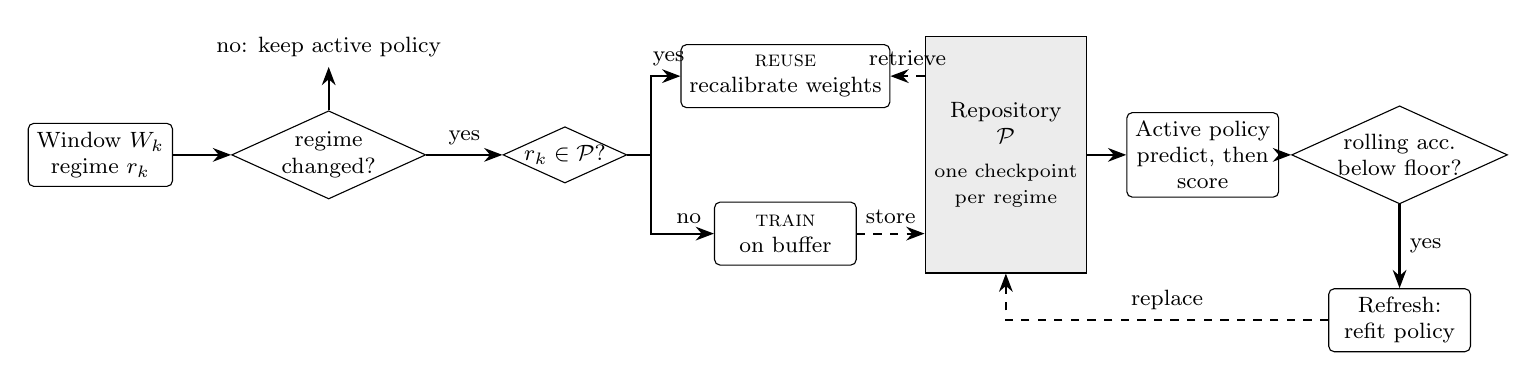
\begin{tikzpicture}[>=Stealth, font=\footnotesize,
  box/.style={draw, rounded corners=2pt, align=center, minimum height=8mm, minimum width=18mm, inner sep=3pt},
  dec/.style={draw, diamond, aspect=2.2, align=center, inner sep=0pt},
  repo/.style={draw, align=center, fill=gray!15, minimum height=30mm, minimum width=19mm},
  flow/.style={->, thick},
  mem/.style={->, dashed, thick}]
\node[box]  (win)  at (0,0)     {Window $W_k$\\regime $r_k$};
\node[dec]  (chg)  at (2.9,0)   {regime\\changed?};
\node[dec]  (hit)  at (5.9,0)   {$r_k \in \mathcal{P}$?};
\node[box]  (reuse) at (8.7,1.0) {\textsc{reuse}\\recalibrate weights};
\node[box]  (train) at (8.7,-1.0){\textsc{train}\\on buffer};
\node[repo] (repo) at (11.5,0)  {Repository\\$\mathcal{P}$\\[1mm]\scriptsize one checkpoint\\\scriptsize per regime};
\node[box]  (act)  at (14.0,0)  {Active policy\\predict, then\\score};
\node[dec]  (mon)  at (16.5,0)  {rolling acc.\\below floor?};
\node[box]  (ref)  at (16.5,-2.1){Refresh:\\refit policy};


\draw[flow] (win) -- (chg);
\draw[flow] (chg) -- node[above]{yes} (hit);
\draw[flow] (chg.north) -- ++(0,0.55) node[above]{no: keep active policy} ;
\draw[flow] (hit.east) -- ++(0.3,0) |- node[pos=0.8,above]{yes} (reuse.west);
\draw[flow] (hit.east) -- ++(0.3,0) |- node[pos=0.8,above]{no} (train.west);
\draw[mem] (repo.west |- reuse.east) -- node[above]{retrieve} (reuse.east);
\draw[mem] (train.east) -- node[above]{store} (repo.west |- train.east);
\draw[flow] (repo.east) -- (act.west);
\draw[flow] (act.east) -- (mon.west);
\draw[flow] (mon.south) -- node[right]{yes} (ref.north);
\draw[mem] (ref.west) -| node[pos=0.25,above]{replace} (repo.south);
\end{tikzpicture}}
\caption{RAPT overview. At each regime boundary the controller looks up the incoming
regime in the repository and either reuses the stored policy or trains and stores a new
one. The active policy predicts and is scored as labels arrive. A monitor refits the
policy and replaces its checkpoint when rolling accuracy degrades. Solid arrows are
control flow, dashed arrows are repository reads and writes.}
\label{fig:overview}
\end{figure}
% ---------- END NEW FIGURE ----------


We represent a regime with its semantic identifier and do not learn a clustering.  What we give up is that
the mechanism requires a usable regime signal; see Section~\ref{sec:limitations}. The
repository holds one checkpoint per regime, made up of the fitted ensemble, its
soft-voting weights, and timestamps for creation and last access. Checkpoints are
immutable.


\subsection{Matching and Transfer}
Matching uses the regime identifier: on a transition to regime $r$, the controller tests
whether $r \in \mathcal{P}$ and retrieves the checkpoint if it does. When reuse goes
ahead, the retrieved ensemble becomes the active policy, and its soft-voting weights are
recalibrated on the most recent buffered window (at most the last 50 observations, skipped
below 20). If no checkpoint exists, a new policy is trained from the class-anchored buffer
and stored. All adaptive models use that buffer in the same way.


\subsection{Monitoring, Refresh, and Fallback}
We use two monitoring rules, and how they differ is one of our findings. The
\emph{absolute} rule triggers when rolling accuracy goes under a fixed floor. The
\emph{relative} rule triggers when accuracy has dropped by more than a fixed margin from
a decayed reference built from that policy's own earlier accuracy. A relative rule cannot
catch a policy that was never good, because the reference decays toward the poor level and
the gap it looks for never appears.

A refresh rebuilds the active policy from the recent buffer and replaces its checkpoint.
In the default refresh the 100-tree ensemble is refit on a 1000-observation buffer; the
cost-aware refresh has the same trigger but refits 20 trees on a 300-observation buffer.

\emph{RAPT-Guard} replaces the indirect degradation monitor with a direct test at the
moment of reuse. When the stream returns to a regime $r$ that already has a checkpoint,
the controller scores the stored ensemble and the prefix-trained ensemble on the most
recent $L$ labelled buffer rows, and reuses the stored policy only if its accuracy is at
least that of the prefix policy plus a margin $m$; otherwise it trains a fresh policy on
the buffer and stores it as the new checkpoint. The gate asks whether reuse is still
better than the fallback we already hold, rather than whether a policy that was never good
has degraded. The lookback is at most one window, so the gate adds one scoring pass per
regime return. We select $(L,m)$ on the development split subject to the reuse rate
staying above $0.30$, so the gate cannot collapse onto ``always train''. RAPT-Enhanced
adds buffer-blended novelty refitting (a 1500-observation buffer instead of 500) and
selective parity refitting (refit a reused policy once its rolling accuracy falls under a
parity threshold for several windows, which reacts only after the stale policy has
predicted, unlike the prospective gate). When no checkpoint exists, or the similarity
gate turns it down, a fresh policy is trained and stored under the incoming regime
identifier.


\section{Experimental Methodology}\label{sec:protocol}
\subsection{Datasets}
Four datasets are summarized in Tab.~\ref{tab:datasets}; all are real network traces.
\emph{5G Campus} is a testbed QoS stream with delay metrics labelled GOOD, DEGRADED or BAD
from the 90th-percentile delay of the next window; 1{,}790 usable samples give 179
windows of 10, each of the three scenarios recurs fourteen times. \emph{UGR'16} is
aggregated ISP netflow with 134 features. Because the calibration split contains almost
no labelled attack traffic, we use the first thirty days of labelled data, one sample per
minute (43{,}200 samples); time-of-day crossed with weekday/weekend gives twelve regimes
and 168 recurrences. \emph{NordicDat} is a cross-border LTE/5G predictive-QoS trace
\cite{nordicdat} whose regimes are operators; it is strongly imbalanced (the smallest
class is $15\%$ of the stream) and is our hardest stream. \emph{5G NR} is a simulated
end-to-end latency stream \cite{nrlatency} of 499 windows of 500 packets across four
regimes (ABCDACBDAB), labelled with the same next-window rule as Campus. Campus and
NordicDat share this three-class next-window delay rule; UGR'16 is binary.


\begin{table}[hbt!]
\small
\caption{Datasets used in evaluations. A window is the adaptation step; 5G NR is one row per window. Recurrences are revisits of an already-seen regime.}
\label{tab:datasets}
\centering
\begin{tabular}{@{}lrrrr@{}}
\toprule
\textbf{Property} & \textbf{Campus} & \textbf{UGR'16} & \textbf{Nordic} & \textbf{5G NR}\\
\midrule
Total samples & 1,799 & 43,200 & 91,455 & 499 \\
Usable samples & 1,790 & 43,200 & 91,000 & 499 \\
Features & 19 & 134 & 16 & 12 \\
Classes & 3 & 2 & 3 & 3 \\
Windows & 179 & 180 & 182 & 499 \\
Samples/window & 10 & 240 & 500 & 1 \\
Regimes & 3 & 12 & 3 & 4 \\
Initial-train windows & 36 & 36 & 36 & 100 \\
\bottomrule
\end{tabular}
\end{table}



\subsection{Preprocessing, Ordering, and Leakage Control} 
All four streams undergo the exact same processing. First, all four streams undergo sorting by row according to timestamp. Then, all identifier and constant columns are dropped. Finally, only those features that are numeric are retained. Any infinite values present within a stream are treated as missing. Any rows that lack a target value are deleted. Any remaining gaps are then filled using medians computed solely from the training prefix. Target thresholds and any scale-related statistics also derive from that prefix. None of the streams are shuffled. The prefix is the first twenty percent of windows: thirty-six for the three cross-dataset streams and ninety-nine for 5G NR. That prefix is completely excluded from evaluation, and that is the sole source of target thresholds. The order of operations is predict → evaluate → adapt for every window prior to its labels being used for adaptation. Regime annotation occurs directly from reading the stream. Therefore, no derivation of annotation can occur based upon the target.


\subsection{Models And Detectors}
Each of the five primary models utilizes exactly the same base architecture and the same retraining buffer. Therefore, any variation between them is due to their respective adaptation mechanisms only. The base is an ensemble of a random forest classifier and an extra-trees classifier, both having fifty trees of depth seven. Frozen is trained once on the prefix and receives no subsequent updates. Event-Driven updates when window accuracy falls below a fixed threshold. Full Retraining rebuilds the model at every regime transition. RAPT, RAPT-Enhanced and RAPT-Guard are the controllers of Section~\ref{sec:method}. We also report two baselines that isolate reuse from the trigger: Frozen+Periodic refits on a fixed five-window schedule, and Event-Driven+Reuse uses the event trigger but retrieves a stored policy when the current regime has one. RAPT-Anchor is an oracle upper bound on the gate: each window it predicts with whichever of the active policy and the prefix policy scored better on the labelled lookback, so its inference cost is doubled and charged as such.


ADWIN, Page-Hinkley, EDD and EDMA operate within the same retraining harness, with identical model, buffer, capacity and minimum-retrain-interval. They differ only by how they detect triggers. Following the finding that the historical default parameters left ADWIN and Page-Hinkley silent, we select their operating points on the development split by a fire-rate criterion (median 5--20 events per stream, with the minimum stream event count maximised) rather than against the evaluation streams. The frozen values are ADWIN $\delta=0.2$; Page-Hinkley $\alpha=0.9999$, $\delta=0.005$, threshold $=0.002$, min-instances $=10$; EDD warning $=2$, drift $=3$; EDMA $\alpha=0.3$, $k=1.5$. All four now consume the per-sample 0/1 error stream, which is the input their original definitions assume. Since none of our streams carry ground-truth drift boundary annotations we report detected events, adaptation cost and predictive performance, not detector precision or recall.


\subsection{Metrics And Statistics}
Performance is evaluated through macro-F1, accuracy, precision and recall. Costs are measured two ways. \emph{Adaptation CPU} is the CPU time devoted to adaptation routines (refits, checkpoint writes, and the gate's scoring passes) and \emph{total CPU} is adaptation plus inference, so a method that infers twice is charged twice. A reduction in adaptation time does not translate proportionally into total runtime, which is why we report both; the total-CPU column is what a deployment actually pays. Each experiment uses thirty seeds (42--71) and we report mean and standard deviation over seeds. Comparisons use the Wilcoxon signed-rank test (paired by window, with Holm correction across the comparison family) and Cohen's $d_z$ on the per-seed paired differences, plus two one-sided tests (TOST) for equivalence at a $\pm0.02$ macro-F1 margin. With thirty seeds the seed-level tests are no longer power-limited; the minimum attainable two-sided $p$-value is $2^{-30}$.


\subsection{Predictive Performance}
Table~\ref{tab:primary} holds the primary comparison. On 5G Campus and 5G NR the models cluster within $0.03$ macro-F1, while UGR'16 and NordicDat separate them sharply. On UGR'16 the frozen baseline is the best model, which is the signature of stale-policy reuse: the regimes recur, but the label relation does not, so retrieving the stored policy is worse than never adapting at all.

\begin{table*}[t]
\caption{Primary comparison, mean over 30 seeds. Bold marks the best macro-F1 per stream; CPU in seconds, retrains and reuses are counts. RAPT-Anchor's total CPU includes its doubled inference.}
\label{tab:primary}
\centering
\scriptsize
\begin{tabular}{@{}llrrrrr@{}}
\toprule
\textbf{Dataset} & \textbf{Model} & \textbf{Macro-F1} & \textbf{Adapt CPU} & \textbf{Total CPU} & \textbf{Retr.} & \textbf{Reuse}\\
\midrule
\multirow{7}{*}{Campus} & Frozen & 0.9371 & 0.000 & 1.185 & 0 & 0 \\
 & Event-Driven & 0.9638 & 0.166 & 1.358 & 1 & 0 \\
 & Full Retraining & $\mathbf{0.9836}$ & 2.192 & 3.375 & 14 & 0 \\
 & RAPT & 0.9385 & 0.281 & 1.452 & 2 & 12 \\
 & RAPT-Enhanced & 0.9385 & 0.279 & 1.431 & 2 & 12 \\
 & RAPT-Guard & 0.9391 & 0.499 & 1.675 & 2 & 12 \\
 & RAPT-Anchor & 0.9385 & 0.282 & 3.893 & 2 & 12 \\
\midrule
\multirow{7}{*}{UGR'16} & Frozen & $\mathbf{0.9693}$ & 0.000 & 1.037 & 0 & 0 \\
 & Event-Driven & 0.8978 & 0.835 & 1.942 & 4 & 0 \\
 & Full Retraining & 0.9511 & 29.771 & 30.872 & 144 & 0 \\
 & RAPT & 0.9137 & 2.571 & 3.640 & 11 & 133 \\
 & RAPT-Enhanced & 0.9137 & 2.595 & 3.669 & 11 & 133 \\
 & RAPT-Guard & 0.9357 & 5.743 & 6.810 & 17 & 127 \\
 & RAPT-Anchor & 0.9247 & 2.595 & 5.683 & 11 & 133 \\
\midrule
\multirow{7}{*}{Nordic} & Frozen & 0.2851 & 0.000 & 1.396 & 0 & 0 \\
 & Event-Driven & 0.2739 & 0.346 & 1.706 & 2 & 0 \\
 & Full Retraining & $\mathbf{0.4376}$ & 3.310 & 4.644 & 19 & 0 \\
 & RAPT & 0.3845 & 0.344 & 1.679 & 2 & 16 \\
 & RAPT-Enhanced & 0.3775 & 3.686 & 5.061 & 21 & 16 \\
 & RAPT-Guard & 0.3793 & 1.154 & 2.537 & 5 & 13 \\
 & RAPT-Anchor & 0.3838 & 0.351 & 4.130 & 2 & 16 \\
\midrule
\multirow{7}{*}{5G NR} & Frozen & 0.9110 & 0.000 & 2.709 & 0 & 0 \\
 & Event-Driven & 0.9081 & 1.312 & 3.984 & 11 & 0 \\
 & Full Retraining & 0.9121 & 0.981 & 3.769 & 8 & 0 \\
 & RAPT & 0.8969 & 0.350 & 3.092 & 3 & 5 \\
 & RAPT-Enhanced & 0.9045 & 0.963 & 3.677 & 8 & 5 \\
 & RAPT-Guard & $\mathbf{0.9148}$ & 0.558 & 3.221 & 4 & 4 \\
 & RAPT-Anchor & 0.9042 & 0.349 & 8.851 & 3 & 5 \\
\bottomrule
\end{tabular}
\end{table*}


On 5G Campus every adaptive model is close to saturation. Full Retraining has the best
macro-F1 ($0.9836$), while RAPT reaches $0.9385$; the gap of $0.0451$ is significant
($p = 1.4 \times 10^{-91}$, $d_z = -12.5$). RAPT-Guard edges it up to $0.9391$, still
$0.0445$ below Full Retraining and still significant. Here the gate is not what is
missing: reuse on this stream brings back a policy that is simply less accurate than one
trained on the current buffer, and the gate correctly prefers the prefix model but the
prefix model is also weaker than Full Retraining.

UGR'16 is where the assumption of the mechanism fails, and it teaches us the most. Frozen
has the highest macro-F1 ($0.9693$). Identity-only reuse is the worst of the eight
primary models: RAPT reaches only $0.9137$, which is $0.0556$ below Frozen
($p = 1.0 \times 10^{-68}$, $d_z = -3.6$) and $0.0375$ below Full Retraining, despite its
133 reuses. The twelve regimes recur and their identifiers stay valid across the 30-day
block, but the netflow-feature-to-attack-label mapping does not stay put. RAPT-Guard,
which validates before reusing, recovers to $0.9357$. That is $0.0220$ above base RAPT
and $0.0336$ below Frozen; both gaps are significant ($p = 9.0 \times 10^{-7}$ and
$p = 1.3 \times 10^{-32}$). So the gate repairs most, but not all, of the damage, and on
this stream it does not beat the frozen baseline. RAPT-Enhanced's parity refit reaches
$0.9137$, the same as base RAPT here, because a policy that is poor from the first reused
window is refit late.

NordicDat is hard to predict and strongly imbalanced. Frozen scores $0.2851$, adaptation
helps, and Full Retraining gets $0.4376$ against $0.3845$ for RAPT, a deficit of $0.0531$
($p = 6.1 \times 10^{-4}$, $d_z = -1.1$). RAPT-Guard scores $0.3793$, $0.0583$ below Full
Retraining. Unlike UGR'16, identity-only reuse here is not catastrophic: RAPT stays above
Frozen ($p = 8.4 \times 10^{-73}$), so reuse is safe on this stream even though it is not
accurate. On 5G NR the models are within $0.03$ of one another and RAPT-Guard has the
best macro-F1 of all methods ($0.9148$), though its edge over Full Retraining ($0.9121$)
is not significant ($p=0.15$). Taken together, the predictive results give no basis for
saying that RAPT improves accuracy. Full Retraining has the best macro-F1 on NordicDat,
the frozen baseline on UGR'16, and a detector baseline on Campus; on 5G NR the best
nominal model is RAPT-Guard. Base RAPT sits below Full Retraining on all four streams. The
case for RAPT is cost, and the case for RAPT-Guard is that it makes reuse safe enough to
use where identity-only reuse is not.

\begin{figure}[t]
\centering
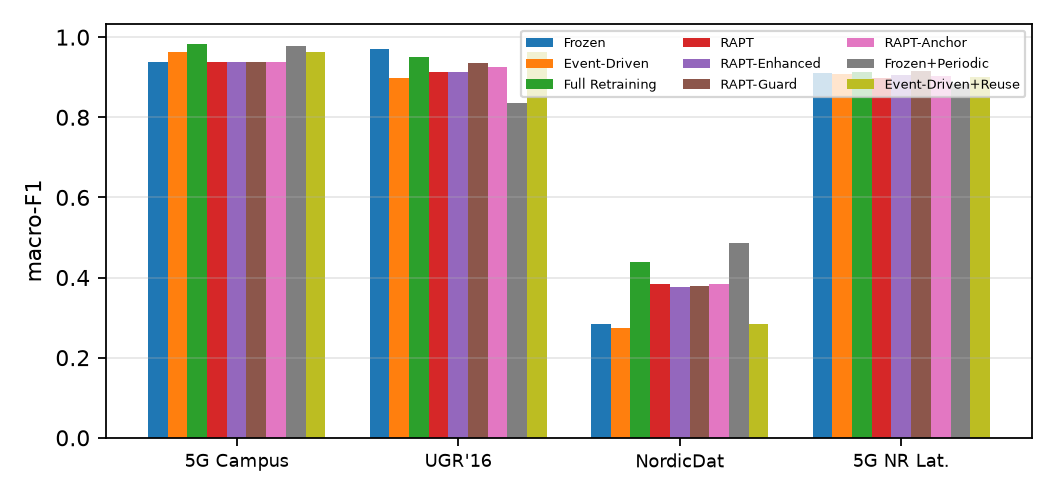
\includegraphics[width=0.7\columnwidth]{primary_performance.png}
\caption{Macro-F1 per method and stream, mean over 30 seeds (Table~\ref{tab:primary}).}
\label{fig:primary}
\end{figure}


\subsection{Computational Cost and Policy Reuse}
Table~\ref{tab:primary} also lists adaptation and total cost
compares total CPU. Relative to Full Retraining the adaptation CPU falls on every stream:
$2.192 \to 0.281$\,s on 5G Campus ($-87.2\%$), $29.771 \to 2.571$\,s on UGR'16
($-91.4\%$), $3.310 \to 0.344$\,s on NordicDat ($-89.6\%$), and $0.981 \to 0.350$\,s on
5G NR ($-64.3\%$). Full Retraining retrains at every regime transition (14, 144, 19 and 8
times); RAPT retrains 2, 11, 2 and 3 times and retrieves a stored policy 12, 133, 16 and
5 times. The gate costs more than identity-only reuse but stays far below Full
Retraining: RAPT-Guard's adaptation CPU is 77.2\%, 80.7\%, 65.1\% and 43.1\% below Full
Retraining on the four streams. The doubled inference of RAPT-Anchor is visible in the
total-CPU column: on 5G NR it totals $8.851$\,s, more than Full Retraining's $3.769$\,s,
even though its adaptation CPU is the lowest of the family. This is why the fair cost
column matters: a method can win on adaptation and lose on total.




\subsection{Efficiency Ablation}
\label{sec:ablation}
On 5G Campus (five seeds) the mechanism ladder is: RAPT-Full $0.9587$ at $0.4283$\,s;
RAPT-Evidence fires \emph{zero} refreshes; RAPT-Floor fires 7.6 refreshes, $0.9797$ at
$0.5865$\,s; RAPT-Cheap $0.9851 \pm 0.0029$ at $0.8477$\,s against Full Retraining
$0.9829 \pm 0.0023$ at $1.4063$\,s ($\Delta=+0.0022$, $p=0.3125$, 95\% interval
$[-0.0036,+0.0080]$ includes zero); RAPT-Incremental $0.9549$ at $0.5813$\,s is worse on
both axes and is dropped. These use the legacy five-seed harness and are power-limited.


\subsection{Validation-Gate Accuracy}
\label{sec:guard}
RAPT-Guard turns every regime return into a decision, so we can audit it. For each return
we compare the gate's choice with the outcome on the incoming window, using a two-point
tolerance: a reuse is harmful only if the stored policy scores more than two points below
the prefix policy, and a block is a miss only if reuse would have been more than two
points better. Table~\ref{tab:gate} reports the counts. The gate almost never allows a
harmful reuse: 0 of 36 on Campus, 6 of 385 on UGR'16 ($1.6\%$), 3 of 39 on NordicDat
($7.7\%$), 0 of 11 on 5G NR; it is slightly conservative on NordicDat, blocking 3 reuses
that would have helped. The zero margin was chosen on the development split to keep the
gate a gate (allow rate above $0.30$) while maximising development macro-F1; a positive
margin blocks almost everything and a negative margin allows everything.

\begin{table}[t]
\caption{RAPT-Guard decisions at every regime return, three seeds, with a two-point tolerance. Bad allow counts a reuse that lost more than two macro-F1 points to the prefix policy on the incoming window.}
\label{tab:gate}
\centering
\footnotesize
\begin{tabular}{@{}lrrrrrr@{}}
\toprule
\textbf{Stream} & \textbf{Returns} & \textbf{Allow} & \textbf{Block} & \textbf{Bad allow} & \textbf{Bad block} & \textbf{Bad-allow rate}\\
\midrule
Campus & 36 & 36 & 0 & 0 & 0 & 0.000 \\
UGR'16 & 399 & 385 & 14 & 6 & 0 & 0.016 \\
Nordic & 48 & 39 & 9 & 3 & 3 & 0.077 \\
5G NR & 15 & 11 & 4 & 0 & 0 & 0.000 \\
\bottomrule
\end{tabular}
\end{table}



\subsection{Comparison to Historical Detectors}
\label{sec:detectors}
Table~\ref{tab:detectors} reports the four historical detectors at the frozen development
operating points; they no longer reduce to the frozen baseline. Page-Hinkley is strongest
on Campus and NordicDat ($0.984$, $0.468$) and matches EDD and EDMA on UGR'16 ($0.960$),
but fires $6$--$34$ times per stream and pays the most adaptation CPU ($2.47$--$5.44$\,s).
ADWIN fires $8.7$ times on UGR'16 and $30$ on NordicDat yet has the weakest NordicDat
macro-F1 ($0.328$): firing more is not adapting well. RAPT fires $2$--$11$ times and
RAPT-Guard $4$--$17$ times, well below the detectors at a fraction of their cost. On
Campus the detectors reach Full-Retraining accuracy at lower cost, so RAPT is not the
accuracy leader there; on UGR'16 the frozen baseline still wins.

\begin{table}[t]
\caption{Historical detectors and the reuse methods at the frozen operating points, mean over 30 seeds. Each cell is macro-F1 with retrain events per seed in parentheses.}
\label{tab:detectors}
\centering
\footnotesize
\begin{tabular}{@{}lrrrr@{}}
\toprule
\textbf{Method} & \textbf{Campus} & \textbf{UGR'16} & \textbf{Nordic} & \textbf{5G NR}\\
\midrule
ADWIN & 0.937 (0.0) & 0.950 (8.7) & 0.328 (30.5) & 0.911 (0.1) \\
Page-Hinkley & 0.984 (6.0) & 0.960 (13.3) & 0.468 (34.1) & 0.905 (19.6) \\
EDD & 0.984 (6.0) & 0.960 (13.3) & 0.433 (32.1) & 0.910 (7.4) \\
EDMA & 0.984 (6.0) & 0.960 (13.3) & 0.378 (29.6) & 0.907 (9.0) \\
Event-Driven & 0.964 (1.0) & 0.898 (3.6) & 0.274 (2.0) & 0.908 (10.9) \\
RAPT & 0.939 (2.0) & 0.914 (11.0) & 0.385 (2.0) & 0.897 (3.0) \\
\bottomrule
\end{tabular}
\end{table}



\subsection{Gate Cadence: Short versus Long Window}
\label{sec:cadence}
The gate can be evaluated on the incoming window only (short, boundary-only lookback) or
on every window while a reused policy is active (long, continuous lookback). Under a
synthetic concept-drift stress panel that reverses the rank order of the top predictive
features inside a regime, the boundary-only cadence never fires a refit, because the drift
is in-regime and there is no boundary to key on; the every-window cadence fires $7$--$10$
refits at the two higher severities. The macro-F1 effect is small where the window is
still predictable ($0.8902 \to 0.8941$ at severity $0.5$, no change at $0.2$ and $1.0$).
The long-window cadence detects in-regime drift the short-window cadence cannot see at
all, but neither moves macro-F1 much once the window is near-single-class, so we claim a
detection mechanism and no large accuracy effect.

\begin{figure}[t]
\centering
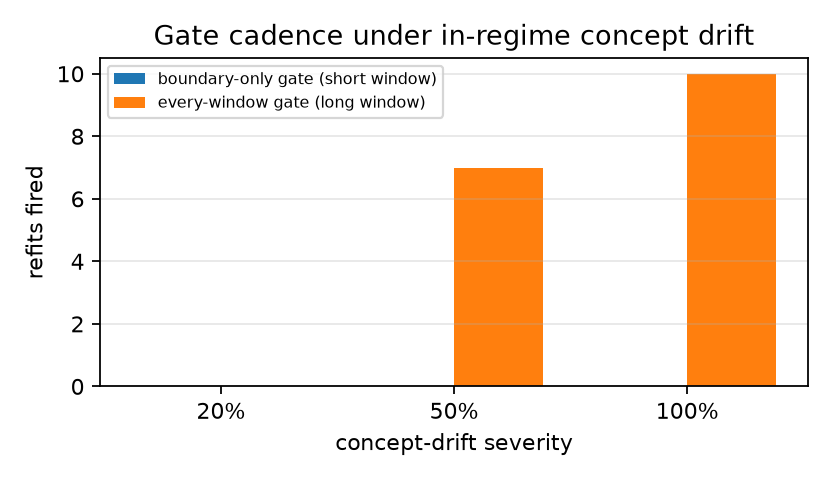
\includegraphics[width=0.62\columnwidth]{gate_cadence.png}
\caption{Short- versus long-window gate under the concept-drift stress panel.}
\label{fig:cadence}
\end{figure}


\section{Discussion}
The mechanism is worth deploying when there is recurrence. The cost saving appears
wherever reuse occurs, but the accuracy penalty is concentrated on UGR'16, where regimes
recur and their label relationship does not. Reusing on the regime identifier alone is
unsafe when label semantics can drift independently of it, and even a direct validation
gate only repairs most of the damage. The practical rule is narrow: reuse when regimes
recur \emph{and} validate the stored policy against the prefix fallback at every return;
if validation finds no stored policy that beats the fallback, do not reuse.


\section{Independent Re-validation}
\label{sec:revalidation}
A harness that re-implements the protocol from the raw per-window records reproduces
Table~\ref{tab:primary} on every predictive metric and regenerates the statistics, gate
counts and detector events; a re-run reproduced every metric exactly but shifted
adaptation CPU by up to $0.14$\,s, so the ordering is stable and the seconds indicative.
Retrieval keys do not track label semantics: an oracle retraining on the previous visit of
the \emph{same} regime reaches only $0.5926$ macro-F1 on UGR'16 against $0.9595$ for Full
Retraining, but $0.9905$ on Campus, exactly where identity-only reuse collapses. The added
controls separate the trigger from reuse: Frozen+Periodic is best on NordicDat ($0.4872$)
and Event-Driven+Reuse best on UGR'16 ($0.9639$), so on UGR'16 the event trigger plus
reuse recovers what identity-keyed reuse loses. A label-delay variant costs RAPT $0.13$
macro-F1 on NordicDat; the headline numbers assume labels arrive with their window.


\section{Limitations and Threats to Validity}
\label{sec:limitations}
The seed-level tests use thirty seeds, so they are not power-limited, but the mechanism
ablation in Section~\ref{sec:ablation} uses five seeds and its smallest two-sided
$p$-value is $0.0625$. Window-level tests assume windows from one stream are independent,
which inflates the effective sample size. The mechanism relies on regime recurrence, which
we measure and do not assume: a stream with no recurrence never exercises the repository,
and a novel regime falls back to retraining with no advantage over the baseline. The
RAPT-Floor threshold and the 20-tree cheap refit were calibrated for this ensemble and
would need revisiting where the pre/post-drift gap is larger. NordicDat stays hard (best
macro-F1 $0.4872$) and we flag it as a hard stream rather than a success. Finally, the
repository is never pruned, and regime similarity is treated as meaningful, which may fail
if the regime signal is noisy.


\section{Conclusion}
Retraining is the standard response to drift, but when conditions return, part of what was
paid for is already in a previously trained model. RAPT keeps one policy per regime and
retrieves it on recurrence, training anew only when no suitable policy exists. Across four
network streams adaptation CPU was 64--91\% below full retraining, while macro-F1 was lower
on all four. Where regimes recurred with changed label relations, identity-only reuse
dropped below even the frozen baseline; RAPT-Guard, which validates the stored policy
against the prefix fallback before every reuse, recovered most of that loss but on UGR'16
still did not beat the frozen baseline. Policy reuse is worth deploying when regimes recur
and the stored policy is validated at every return, and the natural next step is to test
whether a retrieved regime still means what it did when its policy was stored.


\bibliographystyle{IEEEtran}
\bibliography{references}


\end{document}
